\section{Iteración 2}

Una vez que ya tenemos conocimiento extraído de las entrevistas hay que plasmarlo.
Para ello se obtendrán reglas mediante las cuales podamos tomar una decisión, es decir,
crearemos un árbol de decisión el cual sea capaz de llevarnos a una táctica.

Para ello crearemos reglas simples, mediante las cuales con una serie de entradas,
obtendremos una salida. Esta salida puede tener diversas formas. Puede ser una decisión final
o la decisión de un camino intermedio para discernir si elegir una vía u otra.
Estas reglas deberán ser supervisadas por el experto, ya que estas simularan su decisión.

La creación de estas reglas llevarán a un prototipo de sistema experto, el cual será
la primera versión que podrá ser probada en un entorno local para ver si su uso aumenta
el porcentaje de victorias, además del número de tocados dados y a su vez, disminuir el
número de tocados recibidos.

Para ello se empezará con la creación de reglas básicas, como las de la primera entrevista. Esto
nos dará un árbol de decisión que podrá ser ampliable en todo momento.

El primer paso para crear dicho árbol será tener claro cual es el proceso en la toma de decisión.
Para ello se ha creado el diagrama, el cual ha sido corroborado por el experto. Dicho diagrama
se puede observar en la figura 5.4.

\begin{figure}[htb]
  \centering
    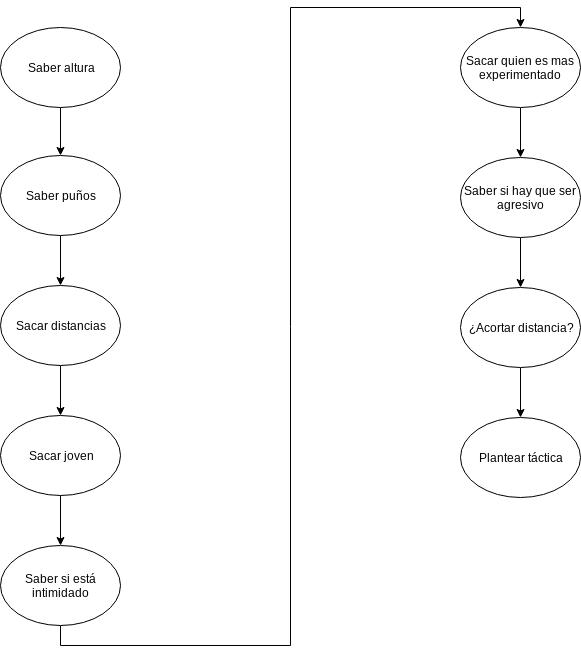
\includegraphics[width=0.8\linewidth]{mapaConocimiento1}
  \caption[Esquema toma decisión]{Esquema toma decisión}
  \label{fig:Esquema toma decisión}
\end{figure}


Con el árbol de decisiones resumido, se elaboraron los sub-arboles para cada uno de los casos.
Estos árboles han sido implantados como diagramas. En la figura 5.5 se puede ver el diagrama
desarrollado para obtener la experiencia. El resto se puede ver en el anexo C donde se encuentran
todos juntos.

\begin{figure}[htb]
  \centering
    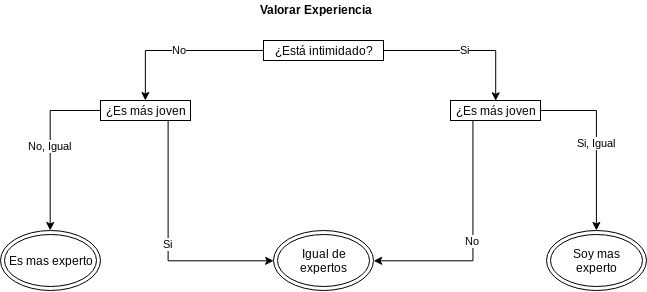
\includegraphics[width=0.8\linewidth]{MapaConocimientoExperiencia}
  \caption[Árbol decisión experiencia]{Árbol decisión experiencia}
  \label{fig:Arbol decisión experiencia}
\end{figure}

Con los los flujos definidos en las tomas de decisión ilustrados mediante diagramas para favorecer
su interpretación y corrección se puede empezar a desarrollar el sistema experto. Para ello inicialzmente
se hará una versión básica de éste mismo que se ampliará poco a poco. Se hará módulo por módulo
para favorecer el desarrollo ágil y una vez listo cada módulo se implementará con el resto.
Al final obtendremos un prototipo del sistema experto desarrollado en CLIPS el cuál será
funcional y podrá ser probado. De este modo conseguiremos pulir fallos en el proceso de desarrollo.

Para ello se han de definir reglas. En el proceso de definición de las reglas se usaron los
diagramas desarrollados anteriormente. A continuación se muestra el desarrollo seguido para el
módulo de experiencia. El diagrama de este módulo se puede ver en la figura 5.5 de este mismo capítulo.

Primero se estudió que variables harían falta. Para ello se definen tres variables las cuales serán booleanas
indicando la altura. Solo una de ellas podrá ser verdadera y siempre habrá una verdadera. Dichas variables son
\textit{ALTOMASEL, ALTOIGUAL} y \textit{ALTOMASYO}. Indicando la primera que el contricante es mas alto, la segunda
que el primer tirador es mas alto mientras que la segunda que ambos son de la misma altura.

Para saber la empuñadura que usa cada tirador se han definido dos variables por tirador. De tal modo que quede como
\text{EMPUÑADURAX} siendo empuñadura el tipo de empuñadura y X el tirador. de modo que las cuatro variables
resultantes son: FRANCESEL, FRANCESYO, ANATOMICOEL y ANATOMICOYO.

Por último para definir quien tiene mas distancia, al igual que con la altura se han definido tres variables.
Estas variables son \textit{MASDISTANCIAEL, DISTANCIAIGUAL} y \textit{MASDISTANCIAYO}. La primera indicaría
que el rival tiene mas distancia, la segunda que ambos tienen la misma distancia, mientras que la última
indicaría que el primer tirador tiene mas distancia.

Con las variables definidas para cada nodo del árbol se definen las reglas, de tal modo que
cuando estén todas definidas, todos los caminos del árbol estén cubiertos. En el cuadro 5.5 se pueden ver
las reglas junto al camino que cubren. Los caminos se pueden ver en la figura 5.6.

\begin{figure}[htb]
  \centering
    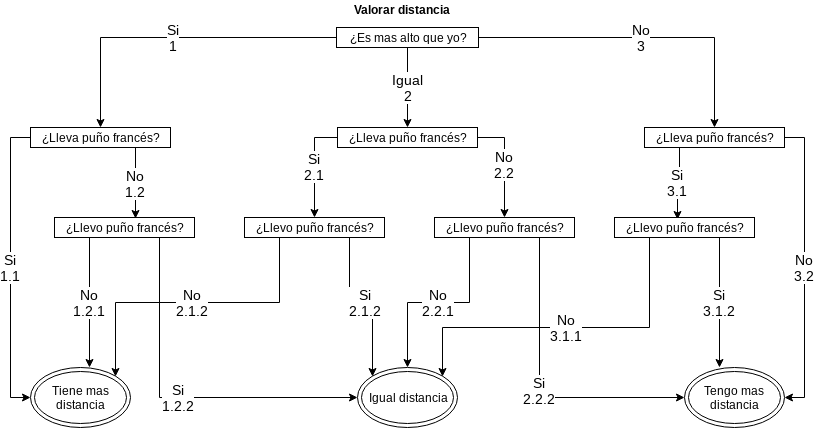
\includegraphics[width=0.8\linewidth]{MapaConocimientoDistanciaCaminos}
  \caption[Arbol decisión distancia con caminos numerados]{Arbol decisión distancia con caminos numerados}
  \label{fig:Arbol decisión distancia con caminos numerados}
\end{figure}

\begin{table}[]
  \centering
  \caption{Reglas distancia}
  \label{tab:Reglas distancia}
  \begin{tabular}{|ll|}
    \hline
    Regla & Camino cubierto \\ \hline
    Si ALTOMASEL y FRANCESEL y FRANCESYO entonces MASDISTANCIAEL & 1.1 \\
    Si ALTOMASEL y ANATOMICOEL y ANATOMICOYO entonces MASDISTANCIAEL & 1.2.1 \\
    Si ALTOMASEL y FRANCESEL y ANATOMICOYO entonces MASDISTANCIAEL & 1.1 \\
    Si ALTOMASEL y ANATOMICOEL y FRANCESYO entonces DISTANCIAIGUAL & 1.2.2 \\
    Si ALTOIGUAL y FRANCESEL y FRANCESYO entonces DISTANCIAIGUAL & 2.1.2 \\
    Si ALTOIGUAL y ANATOMICOEL y ANATOMICOYO entonces DISTANCIAIGUAL & 2.2.1 \\
    Si ALTOIGUAL y FRANCESEL y ANATOMICOYO DISTANCIAMASEL & 2.1.2 \\
    Si ALTOIGUAL y ANATOMICOEL y FRANCESYO entonces DISTANCIAMASYO & 2.2.2 \\
    Si ALTOMASYO y FRANCESEL y FRANCESYO entonces DISTANCIAMASYO & 3.1.2 \\
    Si ALTOMASYO y ANATOMICOEL y ANATOMICOYO entonces DISTANCIAMASYO & 3.2 \\
    Si ALTOMASYO y FRANCESEL y ANATOMICOYO entonces DISTANCIAIGUAL & 3.1.1 \\
    Si ALTOMASYO y ANATOMICOEL y FRANCESYO entonces DISTANCIAMASYO & 3.2 \\ \hline
  \end{tabular}
\end{table}

Con las reglas definidas las pasamos al sistema experto definidas en CLIPS.

A continuación se lista la plantilla y reglas utilizadas para el sistema experto en CLIPS.
\lstinputlisting[keywords={*, defrule, deftemplate, default, slot, type, assert, retract, test}]{code/altura.clp}

El resto de reglas se pueden ver en el anexo D.

Con el prototipo desarrollado era hora de ponerlo a prueba. Recordar que cada uno de los módulos
fue revisado y aprobado por el experto. Para poner a pruebas el prototipo se llevó a la sala de
esgrima de Ciudad Real. Para las pruebas se utilizaron sujetos cuyas características se pueden
ver en el cuadro 5.6.

\begin{table}[]
  \centering
  \caption{Sujetos prueba prototipo}
  \label{tab:Sujetos prueba prototipo}
  \begin{tabular}{|llllll|}
    \hline
    Número de sujeto & Edad & Altura & Años de experiencia & Empuñadura & Naturaleza \\ \hline
    1 & 38 & 160 & 1 año & Frances & Neutra \\ \hline
    2 & 43 & 168 & 1 año y 8 meses & Anatómico & Defensivo \\ \hline
    3 & 23 & 175 & 3 años y 6 meses & Anatómico & Agresivo \\ \hline
    4 & 35 & 183 & 10 años & Anatómico & Defensivo \\ \hline
  \end{tabular}
\end{table}
